\chapter{Introduction}
\label{ch_Introduction}

Real-ESSI is constructed with x2go remote desktop on Amazon Web Service (AWS).
To use the Real-ESSI cloud service, users need to install the x2go client 
on their operating systems.

\section{Install x2go client}
Before connect to Real-ESSI cloud, users should install the client-side of x2go.

\subsection{Install the client-side of x2go}
\paragraph{Install x2go client on Ubuntu} ~

\begin{lstlisting}[frame=single,language=bash]
sudo apt install -y x2goclient
\end{lstlisting}
\paragraph{Install x2go client on Mac}
Users can download the package through this link: 
\url{http://code.x2go.org/releases/X2GoClient_latest_macosx_10_9.dmg}.

\paragraph{Install x2go client on Windows}
Users can download the package through this link: 
\url{http://code.x2go.org/releases/X2GoClient_latest_mswin32-setup.exe}.

\paragraph{Install x2go client on other operating systems}
If you are using a different operating system, please refer to x2go 
website for the installation. The x2go website for client installation 
is \url{https://wiki.x2go.org/doku.php/download:start}

\subsection{Configure the client-side of x2go}

For all operating systems, users will see the same session when they
open the x2goclient new-session, as shown in Fig.~\ref{fig_x2go_client}.

\begin{figure}[H]
  \centering
  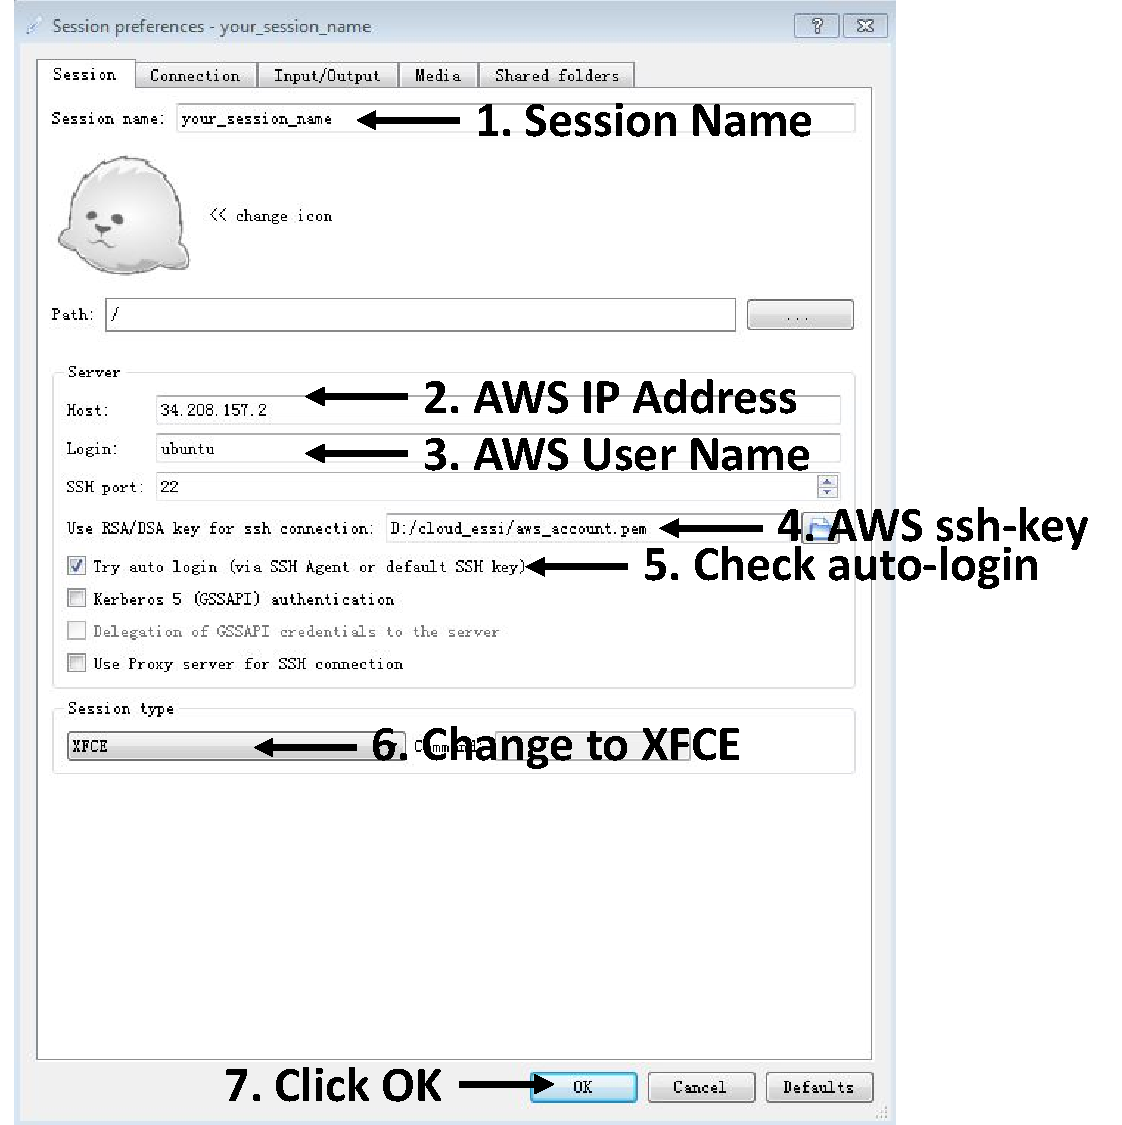
\includegraphics[width = 9cm]{./Figure-files/overview/login_windows_x2go.pdf}
  \caption{Configuration of x2go client}
  \label{fig_x2go_client}
\end{figure}

\begin{enumerate}
	\item Users can name their own session name.
	\item AWS IP address will be provided in the Real-ESSI Short-Course.
	\item AWS User Name is "ubuntu".
	\item AWS ssh-key will be provided in the Real-ESSI Short-Course.
	\item Please check the auto-login.
	\item Please change the session type to XFCE.
	\item Click OK to finish the configuration.
\end{enumerate}

% \section{AWS Regions}

% \subsection{AWS Price by Regions}
% Choosing an AWS region is the first decision you have to make when you set up 
% your AWS components. Most AWS customers choose one based on proximity to 
% themselves or to their end users, which sounds like a sensible thing to do.
% However, proximity alone is not enough.
% The price is also important. 
% An example of AWS price by regions is shown in Fig.~\ref{fig_aws_price_by_regions}. 
% The example is for 10 t2.medium instances running Amazon Linux in the same 
% Availability Zone. Each instance has 20GB of EBS SSD storage. 

% \begin{figure}[H]
%   \centering
%   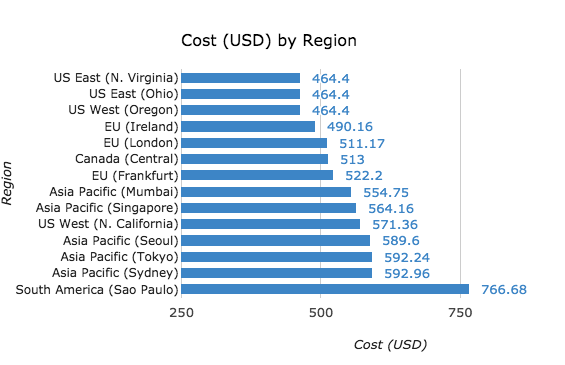
\includegraphics[width = 10cm]{./Figure-files/overview/aws-price-chart.png}
%   \caption{AWS Price by Regions}
%   \label{fig_aws_price_by_regions}
% \end{figure}


% \subsection{AWS Latency by Regions}
% Regions have different latencies and data transfer speeds. 
% An example of AWS latencies by regions is shown in Fig.~\ref{fig_aws_latency_by_regions}.
% The example is a test that measures latency between EC2 instances in different regions.
% For example, from North California it took 2ms to ping EC2 instances in North California,
% and it took 41ms to ping EC2 instances in Oregon.

% \begin{figure}[H]
%   \centering
%   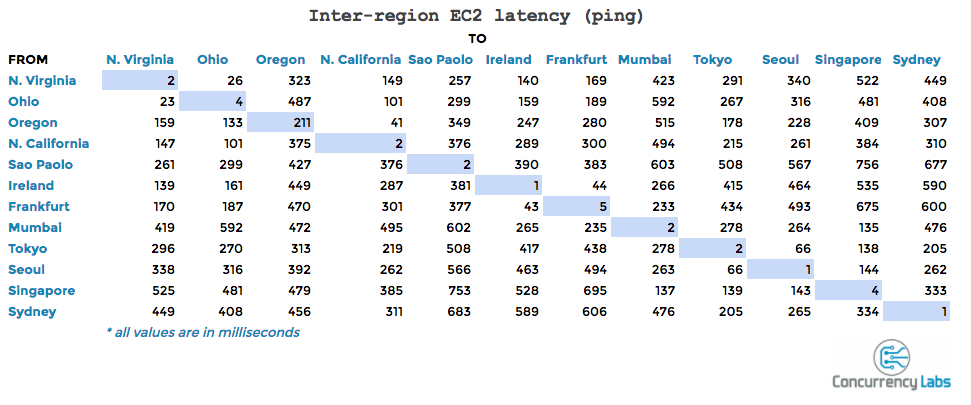
\includegraphics[width = 14cm]{./Figure-files/overview/ec2-ping-table.png}
%   \caption{AWS Latency by Regions}
%   \label{fig_aws_latency_by_regions}
% \end{figure}




